\documentclass[a4paper,11pt]{article}
\usepackage[utf8]{inputenc}
\usepackage[T1]{fontenc}
\usepackage[polish]{babel}
\usepackage{amsmath}
\usepackage{amssymb}
\usepackage{geometry}
\usepackage{graphicx}
\usepackage{multicol}
\geometry{top=0.5in, bottom=0.8in, left=0.8in, right=0.8in}

% Customizable parameters
% Wstaw pełny tytuł zadania
\newcommand{\tasktitle}{Transport}
% Wstaw skrócony tytuł zadania
\newcommand{\taskshort}{TRA}
% Wstaw informacje o konkursie
\newcommand{\contestinfo}{Konkurs Świąteczny 2024 - Grupa Początkująca.}
% Wstaw limit pamięci
\newcommand{\memorylimit}{256 MB}
% Wstaw dane przykładowe wejścia
\newcommand{\exampleinput}{6\\ 3 5 6 1 2 4\\100110}
% Wstaw dane przykładowe wyjścia
\newcommand{\exampleoutput}{2 1 2 2 1 2 }
% Wstaw wyjaśnienie przykładu
\newcommand{\explanation}{Dla $i=1$ ciąg, który otrzymamy przechodząc przez $p$, to i=1 -> i = $p{_1}$ = 3 -> i = $p{_3}$ = 6 ->\\-> i = $p{_6} = 4 -> i = $p{_4} = 1$, zatem widać, że odwiedzimy 2 z nieodwiedzonych państw - pierwsze i czwarte.}
% Wstaw tabelę podzadań
\newcommand{\subtasktable}{% 
\begin{tabular}{|c|c|c|}
\hline
Podzadanie & Ograniczenia & Punkty \\
\hline
1 & permutacja $p$ składa się z kolejnych elementów & 5\\
2 & $n \leq 10^3$ & 25 \\
3 & brak dodatkowych ograniczeń & 70 \\
\hline
\end{tabular}}

\begin{document}

% Nagłówek zadania
\noindent\textbf{\LARGE Zadanie: \taskshort} \\
\textbf{\Large \tasktitle} \\
\rule{\textwidth}{0.4pt} \\
\small \contestinfo \
\textbf{Dostępna pamięć: \memorylimit.}

% Wstaw obrazek
\begin{center}
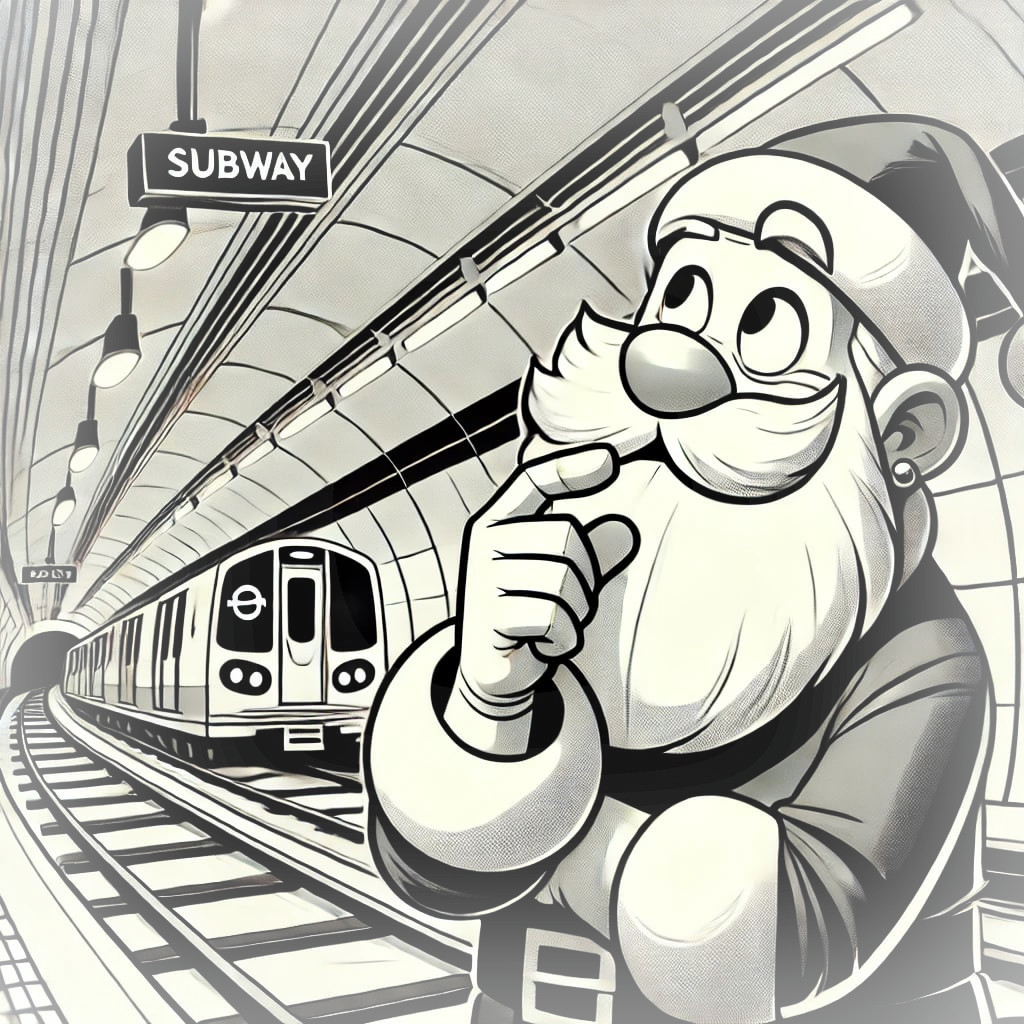
\includegraphics[width=0.6\textwidth]{transport_zdj_1.jpeg} % Zmień "zdj.png" na nazwę pliku z obrazkiem
\end{center}

% Treść zadania
\noindent Mikołaj rozwozi prezenty do $n$ państw oznaczonych od 1 do $n$. Istnieje jednak podziemna kolej szybkiego transportu, która pozwala na znaczne przyspieszenie czasu podróży oraz zaoszczędzenie na kosztach przemieszczania (ponieważ Mikołaj w okresie świątecznym płaci jedyną uczciwą kwotę, czyli 0zł). Jej linie określone są przez permutację $p$, która mówi, że z państwa $i$ do państwa $j$ można dostać się wtedy, gdy jest możliwe uzyskanie równości $i=j$ poprzez przypisywanie $i$ kolejnych wartości $p{_i}$ wymaganą ilość razy. Dodatkowo elfy prowadzą skrupulatną listę odwiedzonych już państw (1 oznacza państwo odwiedzone, a 0 - nieodwiedzone). Kancelaria Świętego Mikołaja prosi cię o napisanie programu, który dla każdego kraju $i$ wyznaczy do ilu nieodwiedzonych jeszcze państw będzie można się z niego dostać za darmo, bez korzystania z sań.

% Sekcja wejścia
\section*{Wejście}
Pierwszy wiersz wejścia zawiera liczbę $n$ ($1 \leq n \leq 10^6$), oznaczającą liczbę państw.\\\\Drugi wiersz zawiera $n$ liczb $p{_1}$, $p{_2}$,..., $p{_n}$ ($1 \leq p{_i} \leq n$) będące kolejnymi elementami permutacji $p$.\\\\W kolejnym wierszu zapisany jest ciąg $s$ składający się z elementów '0' i '1', gdzie 1 oznacza państwo odwiedzone, a 0 nieodwiedzone.

% Sekcja wyjścia
\section*{Wyjście}
Dla każdej liczby $i$ od 1 do $n$ wypisz ile nieodwiedzonych państw Mikołaj będzie mógł odwiedzić za darmo, jeżeli rozpocznie swoją podróż w państwie $i$.
\newpage
% Sekcja przykładów
\section*{Przykład}
\begin{multicols}{2}
\noindent\textbf{Wejście:} \\
\exampleinput

\columnbreak

\noindent\textbf{Wyjście:} \\
\exampleoutput
\end{multicols}

\noindent Wyjaśnienie: \explanation

% Sekcja oceniania
\section*{Ocenianie}
Zestaw testów dzieli się na następujące podzadania:
\begin{center}
\subtasktable
\end{center}

% Stopka
\vspace*{\fill}
\noindent\rule{\textwidth}{0.4pt} \\
\small \textbf{Autor:} Filip Nowak, Antoni Iwanowski \hfill \textbf{VIII LO im. Władysława IV w Warszawie}

% Komentarze:
% W polu \tasktitle wpisz pełny tytuł zadania.
% W polu \taskshort wpisz skrócony tytuł zadania.
% W polu \contestinfo wpisz informacje o konkursie.
% W polu \memorylimit wpisz limit pamięci.
% W polach \exampleinput i \exampleoutput wpisz dane przykładowe wejścia i wyjścia.
% W polu \explanation wpisz wyjaśnienie przykładu.
% W polu \subtasktable wpisz tabelę z podzadaniami, ich ograniczeniami i punktami.
% W stopce wstaw autora i nazwę szkoły.
\end{document}
